\Variant{02.10.2026 (2-smena)}
\QQ{1}{$\overline{abab}$ tört xonali son bölib, $a$ va $b$ — raqamlar ($a\ne0$). Bu son quyidagilardan qaysi biriga har doim qoldiqsiz bölinadi?
\Opts{$11$}{$101$}{$111$}{$100$}}
\QQ{2}{Hisoblang:
\[\frac{3-\dfrac1{\frac12-1}}{3+\dfrac1{\frac12+1}}\]
\Opts{$\dfrac{15}{11}$}{$\dfrac7{11}$}{$\dfrac{11}{15}$}{$\dfrac5{11}$}}
\QQ{3}{Soat 03:00 ni körsatmoqda. Neça minutdan söng soat va minut millari ustma-ust tuşadi?
\Opts{$15$}{$16\dfrac5{11}$}{$17\dfrac3{11}$}{$16\dfrac4{11}$}}
\QQ{4}{Anvar oylik maoşining $40\%$ i, Abror esa oylik maoşining $30\%$ i miqdorida qöşimça haq oldi. Anvarning oylik maoşi Abrornikidan $500\,000$ söm köp. Anvar olgan qöşimça haq Abror olganidan $350\,000$ söm köp bölsa, Abror qança qöşimça haq olgan?
\Opts{$350\,000$ söm}{$400\,000$ söm}{$450\,000$ söm}{$500\,000$ söm}}
\QQ{5}{Soddalaştiring:
\[\left(a^{\frac23}b^{-\frac12}\right)^3\cdot\left(a^{-\frac12}b^{\frac34}\right)^2:\left(a^{\frac13}b^{\frac16}\right)^3\]
\Opts{$\dfrac1{\sqrt b}$}{$\dfrac a{\sqrt b}$}{$\sqrt a$}{$a\sqrt b$}}
\QQ{6}{Hisoblang:
\[\frac{2+\sqrt3}{\sqrt2+\sqrt{2+\sqrt3}}+\frac{2-\sqrt3}{\sqrt2-\sqrt{2-\sqrt3}}\]
\Opts{$\sqrt2$}{$2-\sqrt2$}{$1$}{$2+\sqrt2$}}
\QQ{7}{Soddalaştiring:
\[\sqrt[4]{\sqrt7-\sqrt[4]{24}}\cdot\sqrt{1+\sqrt6}\cdot\sqrt[4]{\sqrt7+\sqrt[4]{24}}\]
\Opts{$5$}{$1$}{$\sqrt7$}{$\sqrt5$}}
\QQ{8}{Arifmetik progressiyaning hadlari uçun $a_1+a_3+a_5+a_7=40$ va $a_2+a_4+a_6+a_8=51$ bölsa, $a_{10}$ ni toping.
\Opts{$25$}{$26{,}5$}{$27{,}5$}{$24$}}
\QQ{9}{$\{a_n\}$ arifmetik progressiyaning dastlabki uçta hadi yiğindisi $15$ ga teng. Quyidagiça yangi sonlar tuzilgan: $b_1=a_1$, $b_2=a_2+1$, $b_3=a_3+5$. Agar $b_1$, $b_2$, $b_3$ kamayuvçi geometrik progressiya taşkil qilsa, $b_1+b_2+b_3$ yiğindini toping.
\Opts{$21$}{$18$}{$24$}{$12$}}
\QQ{10}{Agar $a=2{,}2$ va $b=1{,}1$ bölsa, $a^3-b^3-3ab(a-b)$ ning qiymatini toping.
\Opts{$1{,}21$}{$1{,}1$}{$3{,}993$}{$1{,}331$}}
\QQ{11}{$x^8+x^4+1$ va $x^5+x+1$ köphadlarning EKUBini toping.
\Opts{$x^2-x+1$}{$x^2+x+1$}{$x^3-1$}{$x-1$}}
\QQ{12}{Soddalaştiring:
\[\sin^2\alpha\cdot\tg^2\alpha+\cos^2\alpha\cdot\ctg^2\alpha+3\]
\Opts{$\dfrac1{\sin^22\alpha}$}{$\tg^2\alpha+\ctg^2\alpha$}{$\dfrac4{\sin^22\alpha}$}{$4$}}
\QQ{13}{Hisoblang:
\[2\sqrt2\sin\left(\frac\pi2+\arctg\sqrt7\right)\]
\Opts{$1$}{$\sqrt7$}{$0$}{$3$}}
\QQ{14}{Tenglamaning haqiqiy ildizlari yiğindisini toping:
\[5^{x-1}+5\cdot0{,}2^{x-2}=26\]
\Opts{$3$}{$4$}{$2$}{$5$}}
\QQ{15}{Tengsizlikning butun yeçimlari sonini toping:
\[x^{\frac12}-3x^{\frac14}+2\le0\]
\Opts{$16$}{$15$}{$17$}{$14$}}
\QQ{16}{Tenglamaning haqiqiy ildizlari yiğindisini toping (agar tenglama bitta ildizga ega bölsa, şu ildizni toping):
\[\sqrt{2x+7}=x+2\]
\Opts{$1$}{$-2$}{$-3$}{$4$}}
\QQ{17}{Agar $N=\dfrac16\left((\log_224)^3-(\log_26)^3-(\log_212)^3+(\log_23)^3\right)$ bölsa, $2^N$ ni toping.
\Opts{$36$}{$48$}{$24$}{$72$}}
\QQ{18}{Tenglamaning haqiqiy ildizlari yiğindisini toping:
\[x^2+4x-5|x+2|-2=0\]
\Opts{$-4$}{$4$}{$-8$}{$0$}}
\QQ{19}{Tengsizlikning butun yeçimlari yiğindisini toping:
\[(x-3)\cdot\log_2(x-1)\le0\]
\Opts{$5$}{$2$}{$3$}{$6$}}
\QQ{20}{$f(x)=ax^3+bx^2+cx$ funksiya uçun $f(1)=1$, $f(2)=2$, $f(3)=4$ bölsa, $f(5)$ ni toping.
\Opts{$25$}{$15$}{$5$}{$65$}}
\QQ{21}{Rasmda
\[f(x)=\begin{cases}\log_2(x-b), & x>a,\\ |x|+c, & x\le a\end{cases}\]
funksiya grafigi berilgan. $f(a)$ ni toping.
\qfig{\begin{tikzpicture}[scale=0.55,font=\small]
\draw[-{Stealth[length=4pt]}] (-3.5,0)--(7.6,0) node[right] {$x$}; \draw[-{Stealth[length=4pt]}] (0,-3.5)--(0,5) node[left] {$y$};
\draw[gray,dashed] (1,-6)--(1,5);
\draw[thick] (-3,4)--(0,1)--(1,2); \fill (1,2) circle (3pt);
\draw[thick,domain=1.016:7,samples=100] plot (\x,{ln(\x-1)/ln(2)}) node[above right] {$y=f(x)$};
\fill (5,2) circle (2.5pt); \node[above left] at (5,2) {$(5;\,2)$};
\node[left] at (0,1) {$1$}; \node[below left] at (0,0) {$O$}; \node[below right] at (2,0) {$2$};
\end{tikzpicture}}
\Opts{$2$}{$1$}{$0$}{$3$}}
\QQ{22}{$f(x)=\dfrac{8^x+4^x+3\cdot2^x}{\ln2}$ funksiya berilgan. $f'(x_0)$ ni toping, bunda $x_0=\log_23$.
\Opts{$96$}{$120$}{$81$}{$108$}}
\QQ{23}{$f(x)=\dfrac2{\sqrt{2-x^2}}$ funksiyaning grafigi $(-1;\,0)$ nuqtadan ötuvçi boşlanğiç funksiyasini toping.
\Opts{$2\arccos\dfrac x{\sqrt2}-\dfrac\pi2$}{$2\arccos\dfrac x{\sqrt2}+\dfrac\pi2$}{$2\arcsin\dfrac x{\sqrt2}+\dfrac\pi2$}{$2\arcsin\dfrac x{\sqrt2}-\dfrac\pi2$}}
\QQ{24}{Tomonlari $12$ va $9$ ga teng bölgan töğri törtburçak içiga uçta özaro urinuvçi aylana çizilgan. Pastki ikkita aylananing radiuslari teng bölib, ular töğri törtburçakning pastki asosiga hamda mos ravişda çap va öng yon tomonlariga urinadi. Yuqoridagi uçinçi aylana esa töğri törtburçakning yuqori asosiga urinadi. Kiçik aylananing uzunligini toping.
\qfig{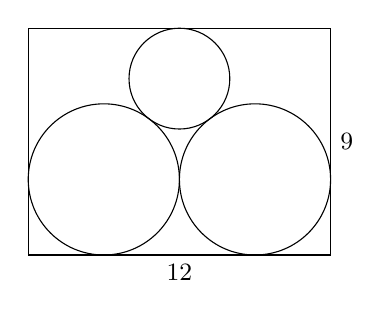
\begin{tikzpicture}[scale=0.32,font=\small]
\draw (0,0) rectangle (12,9); \draw (3,3) circle (3); \draw (9,3) circle (3); \draw (6,7) circle (2);
\node[below] at (6,0) {$12$}; \node[right] at (12,4.5) {$9$};
\end{tikzpicture}}
\Opts{$3\pi$}{$4\pi$}{$2\pi$}{$5\pi$}}
\QQ{25}{$ABC$ uçburçakning tomonlari $AB=8$, $BC=10$ va $AC=12$ ga teng. Uçburçakka içki çizilgan aylanaga ötkazilgan urinma $AC$ va $BC$ tomonlarni mos ravişda $E$ va $F$ nuqtalarda kesib ötadi. Hosil bölgan $EFC$ uçburçakning perimetrini toping.
\qfig{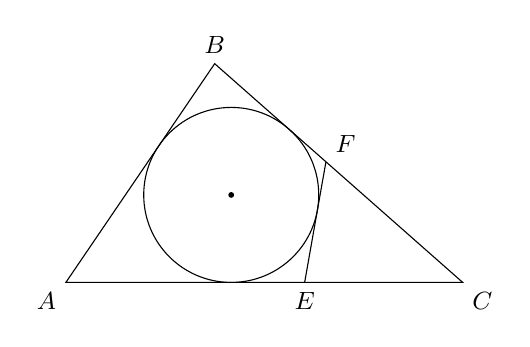
\begin{tikzpicture}[scale=0.42,font=\small]
\coordinate (A) at (0,0); \coordinate (C) at (12,0); \coordinate (B) at (4.5,6.614); \coordinate (I) at (5,2.646); \coordinate (E) at (7.22,0); \coordinate (F) at (7.864,3.647);
\draw (A)--(B)--(C)--cycle; \draw (I) circle (2.646); \draw (E)--(F); \fill (I) circle (2.5pt);
\node[below left] at (A) {$A$}; \node[above] at (B) {$B$}; \node[below right] at (C) {$C$}; \node[below] at (E) {$E$}; \node[above right] at (F) {$F$};
\end{tikzpicture}}
\Opts{$14$}{$10$}{$12$}{$16$}}
\QQ{26}{Tomonlari $8$ va $6$ ga teng bölgan töğri törtburçak diagonali orqali ikkita töğri burçakli uçburçakka ajratildi va ularga aylanalar içki çizildi. Uşbu aylanalarning diagonal bilan uriniş nuqtalari orasidagi $x$ masofani toping.
\qfig{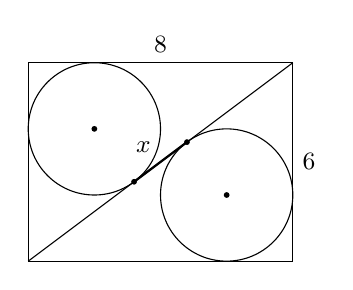
\begin{tikzpicture}[scale=0.42,font=\small]
\draw (0,0) rectangle (8,6); \draw (0,0)--(8,6); \draw (2,4) circle (2); \draw (6,2) circle (2);
\fill (2,4) circle (2.5pt); \fill (6,2) circle (2.5pt); \draw[thick] (3.2,2.4)--(4.8,3.6); \fill (3.2,2.4) circle (2.5pt); \fill (4.8,3.6) circle (2.5pt);
\node[above left] at (4,3) {$x$}; \node[above] at (4,6) {$8$}; \node[right] at (8,3) {$6$};
\end{tikzpicture}}
\Opts{$5$}{$3$}{$2{,}5$}{$2$}}
\QQ{27}{$ABCD$ töğri törtburçakda $AB=13$. $DC$ tomonda $E$ nuqta olingan bölib, $AE=12$ va $\angle AEB=90^\circ$. $EBC$ uçburçakning yuzi $S$ ni toping.
\qfig{\begin{tikzpicture}[scale=0.42,font=\small]
\coordinate (A) at (0,0); \coordinate (B) at (13,0); \coordinate (C) at (13,4.615); \coordinate (D) at (0,4.615); \coordinate (E) at (11.077,4.615);
\fill[qfill] (E)--(B)--(C)--cycle;
\draw (A)--(B)--(C)--(D)--cycle; \draw (A)--(E)--(B);
\draw ($(E)!0.6cm!(A)$)--($(E)!0.6cm!(A)+(E)!0.6cm!(B)-(E)$)--($(E)!0.6cm!(B)$);
\node[below left] at (A) {$A$}; \node[below right] at (B) {$B$}; \node[above right] at (C) {$C$}; \node[above left] at (D) {$D$}; \node[above] at (E) {$E$};
\node[above] at (5.5,2.4) {$12$}; \node[below] at (6.5,0) {$13$}; \node at (12.3,2.9) {$S$};
\end{tikzpicture}}
\Opts{$30$}{$\dfrac{750}{169}$}{$\dfrac{60}{13}$}{$\dfrac{4320}{169}$}}
\QQ{28}{$ABCDEFGHIJ$ muntazam önburçak berilgan. $BG$ va $CG$ diagonallari orasidagi burçakni toping.
\qfig{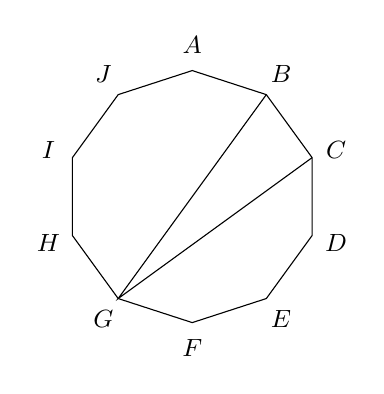
\begin{tikzpicture}[scale=1.6,font=\small]
\foreach \n/\a in {A/90,B/54,C/18,D/-18,E/-54,F/-90,G/-126,H/-162,I/162,J/126} {\coordinate (\n) at (\a:1); \node at (\a:1.2) {$\n$};}
\draw (A)--(B)--(C)--(D)--(E)--(F)--(G)--(H)--(I)--(J)--cycle; \draw (B)--(G)--(C);
\end{tikzpicture}}
\Opts{$18^\circ$}{$12^\circ$}{$24^\circ$}{$36^\circ$}}
\QQ{29}{$A(1;\,2)$ va $B(5;\,-2)$ nuqtalar berilgan. $AB$ kesmaning örta perpendikulyari tenglamasini toping.
\Opts{$y=x-3$}{$y=-x+3$}{$y=x+3$}{$y=2x-6$}}
\QQ{30}{$A$ nuqtadan tekislikka $AC$ va $AB$ oğmalar hamda $AH$ perpendikulyar tuşirilgan. $AC$ oğma tekislik bilan $30^\circ$, $AB$ oğma esa $45^\circ$ li burçak hosil qiladi. Agar $AH=5$ bölsa, $BC$ kesmaning eng kiçik uzunligini toping.
\Opts{$5\left(\sqrt3+1\right)$}{$5\left(\sqrt3-1\right)$}{$5\sqrt2$}{$10$}}
\QQ{31}{9-A sinfda $30$ ta öquvçi bor. Ulardan $14$ tasi matematika, $18$ tasi ingliz tili tögaragiga boradi. Agar sinfdagi öquvçilarning $20\%$ i heç qaysi tögarakka bormasa, neçta öquvçi faqat matematika tögaragiga boradi?
\Opts{$10$}{$12$}{$6$}{$8$}}
\QQ{32}{$4$ ta oddiy kubik bir vaqtda taşlandi. Kamida bitta kubikning ustki tomonida $3$ raqami tuşiş ehtimoli neçaga teng?
\Opts{$\dfrac{625}{1296}$}{$\dfrac1{1296}$}{$\dfrac{125}{324}$}{$\dfrac{671}{1296}$}}
\QQ{33}{\Moslash{Tomonlari $13$, $14$ va $15$ bölgan uçburçak uzunligi $14$ ga teng tomoni atrofida $360^\circ$ ga aylantirildi.
\par\centering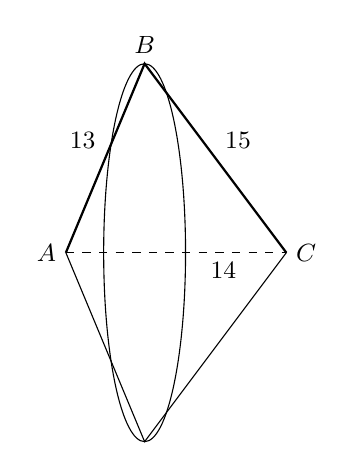
\begin{tikzpicture}[scale=0.2,font=\small]
\draw (0,0)--(5,12)--(14,0)--(5,-12)--cycle; \draw (5,0) ellipse (2.6 and 12); \draw[dashed] (0,0)--(14,0);
\draw[thick] (0,0)--(5,12)--(14,0);
\node[left] at (0,0) {$A$}; \node[right] at (14,0) {$C$}; \node[above] at (5,12) {$B$};
\node[above left] at (2.5,6) {$13$}; \node[above right] at (9.5,6) {$15$}; \node[below] at (10,0) {$14$};
\end{tikzpicture}}{A) $33$\par B) $336\pi$\par C) $34$\par D) $672\pi$\par E) $35$\par F) $288\pi$}{Hosil bölgan jismning töla sirtini toping.}{Hosil bölgan jismning hajmini toping.}{Hosil bölgan jismga içki çizilgan şar hajmini toping.}}
\QQ{36}{Tenglamani yeçing:
\[\left(9-x^2\right)^4+\left(7-x^2\right)^4=16\]
\AB{Tenglama neçta haqiqiy ildizga ega?}{Tenglamaning haqiqiy ildizlari köpaytmasini toping.}}
\QQ{37}{Tenglamani yeçing:
\[37\tg3x=11\tg x\]
\AB{Tenglamaning $(-\pi;\,\pi)$ oraliqdagi yeçimlari sonini toping.}{Tenglamaning $[-\pi;\,\pi]$ oraliğidagi eng katta va eng kiçik ildizlari yiğindisini toping.}}
\QQ{38}{$f(x)$ funksiya $x\ne0$ uçun aniqlangan va $f(x)+3f\left(\dfrac1x\right)=4x$ tenglikni qanoatlantiradi.
\AB{$f(2)$ ni hisoblang.}{$f(x)=0$ tenglama neçta ildizga ega?}}
\QQ{39}{$f(x)=e^{2x-a}$ va $g(x)=\dfrac{\ln x+a}2$ funksiyalar berilgan.
\qfig{\begin{tikzpicture}[scale=0.55,font=\small]
\draw[-{Stealth[length=4pt]}] (-5,0)--(5,0) node[right] {$x$}; \draw[-{Stealth[length=4pt]}] (0,-4)--(0,4) node[left] {$y$};
\draw[thick,domain=-4.5:-1.2,samples=60] plot (\x,{exp(2*\x+3)}); \node[above left] at (-2,1) {$y=f(x)$};
\draw[thick,domain=0.2:4.5,samples=60] plot (\x,{(ln(\x)-3)/2}); \node[below right] at (1.5,-1.5) {$y=g(x)$};
\node[below left] at (0,0) {$O$};
\end{tikzpicture}}
\AB{$a=-3$ bölganda bu funksiyalar grafiklari orasidagi eng qisqa masofani toping.}{$a$ ning qanday qiymatida bu funksiyalar grafiklari urinadi?}}
\QQ{40}{$f(x)=ax^2+bx+c$ parabola $Ox$ öqini $(3;\,0)$ va $F(-4;\,0)$ nuqtalarda, $Oy$ öqini $E(0;\,12)$ nuqtada kesadi. Parabolaga $EF$ töğri çiziqqa parallel urinma ötkazildi, $M(x_0;\,y_0)$ — uriniş nuqtasi.
\qfig{\begin{tikzpicture}[xscale=0.7,yscale=0.3,font=\small]
\fill[qfill] (-16/3,0)--(-2,10)--plot[domain=-2:-4,samples=30] (\x,{-(\x+4)*(\x-3)})--cycle;
\draw[-{Stealth[length=4pt]}] (-7,0)--(5,0) node[right] {$x$}; \draw[-{Stealth[length=4pt]}] (0,-4)--(0,15) node[left] {$y$};
\draw[thick,domain=-4.6:4,samples=80] plot (\x,{-(\x+4)*(\x-3)});
\draw[domain=-4.8:0.7,samples=2] plot (\x,{3*\x+12}); \draw[domain=-6.5:-0.6,samples=2] plot (\x,{3*\x+16});
\draw[dashed] (-2,0)--(-2,10)--(0,10);
\fill (-2,10) circle (3pt); \fill (0,12) circle (3pt); \fill (-4,0) circle (3pt);
\node[left] at (-2.7,10.6) {$M(x_0;\,y_0)$}; \node[right] at (0.1,12.6) {$E(0;\,12)$}; \node[below left] at (-4.1,-1.1) {$F(-4;\,0)$}; \node[above right] at (3,0) {$3$}; \node[below right] at (0,0) {$O$};
\end{tikzpicture}}
\AB{$x_0+y_0$ ni toping.}{Böyalgan soha yuzini toping.}}
\QQ{41}{$ABC$ uçburçakning $AB$ tomonida $D$ va $E$ nuqtalar, $AC$ tomonida $F$ nuqta olingan. Bunda $\dfrac{DB}{AB}=\dfrac17$, $\dfrac{AF}{AC}=\dfrac12$, $AE=4$, $DE=8$, $FC=3$ va $\angle BAC=60^\circ$.
\qfig{\begin{tikzpicture}[scale=0.42,font=\small]
\coordinate (A) at (0,0); \coordinate (C) at (6,0); \coordinate (B) at (7,12.124); \coordinate (D) at (6,10.392); \coordinate (E) at (2,3.464); \coordinate (F) at (3,0);
\draw (A)--(B)--(C)--cycle; \draw (D)--(C); \draw (E)--(F);
\draw ($(A)+(0:0.9)$) arc[start angle=0,end angle=60,radius=0.9]; \node at ($(A)+(30:1.5)$) {\scriptsize$60^\circ$};
\node[left] at (A) {$A$}; \node[above] at (B) {$B$}; \node[right] at (C) {$C$}; \node[left] at (D) {$D$}; \node[left] at (E) {$E$}; \node[below] at (F) {$F$};
\node[left] at (1,1.9) {$4$}; \node[left] at (4,7) {$8$}; \node[below] at (4.5,0) {$3$};
\end{tikzpicture}}
\AB{$BDC$ uçburçakning yuzini toping.}{$CDEF$ törtburçakning yuzini toping.}}
\QQ{42}{Qirrasi $6$ cm bölgan özaro teng $3$ ta kub rasmdagidek ustma-ust piramida şaklida joylaştirilgan, bunda yuqoridagi kub ostidagi kublarning teng yarmida yotadi.
\qfig{\begin{tikzpicture}[scale=0.3,font=\small]
\coordinate (A) at (0,6); \coordinate (B) at (6,12); \coordinate (C) at (12,0);
\draw (0,0) rectangle (6,6); \draw (6,0) rectangle (12,6); \draw (3,6) rectangle (9,12);
\draw (A)--(B)--(C)--cycle; \draw (7.5,5.7)--(7.5,6.3); \draw (10.5,5.7)--(10.5,6.3);
\draw ($(A)+(0:1.2)$) arc[start angle=0,end angle=45,radius=1.2]; \node at ($(A)+(22:1.8)$) {\scriptsize$\alpha$};
\node[left] at (A) {$A$}; \node[above] at (B) {$B$}; \node[below right] at (C) {$C$};
\end{tikzpicture}}
\AB{$\alpha$ burçakni toping.}{$ABC$ uçburçak yuzini toping.}}
\QQ{43}{$ABCDE$ beşburçakka radiusi $2$ ga teng aylana taşqi çizilgan. Bunda $\angle ABE=45^\circ$, $\angle EBD=45^\circ$, $AB=2$ va $BC=CD$.
\qfig{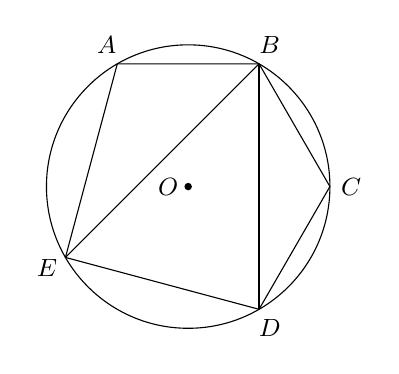
\begin{tikzpicture}[scale=0.9,font=\small]
\draw (0,0) circle (2);
\foreach \n/\a in {A/120,B/60,C/0,D/-60,E/-150} {\coordinate (\n) at (\a:2); \node at (\a:2.3) {$\n$};}
\draw (A)--(B)--(C)--(D)--(E)--cycle; \draw (B)--(E); \draw (B)--(D); \fill (0,0) circle (1.5pt); \node[left] at (0,0) {$O$};
\end{tikzpicture}}
\AB{Beşburçakning perimetrini toping.}{Beşburçakning yuzini toping.}}
\QQ{44}{Konusning töla sirti asos yuzidan $4$ marta katta, hajmi esa $72\pi$ ga teng. Konusga şar içki çizilgan.
\qfig{\begin{tikzpicture}[scale=0.3,font=\small]
\coordinate (S) at (0,12); \coordinate (A) at (-4.243,0); \coordinate (B) at (4.243,0); \coordinate (O) at (0,0);
\shade[ball color=qfill!60,opacity=0.7] (0,3) circle (3); \draw (0,3) circle (3); \draw (-3,3) arc (180:360:3 and 0.7); \draw[dashed] (3,3) arc (0:180:3 and 0.7);
\draw (A)--(S)--(B); \draw (-4.243,0) arc (180:360:4.243 and 1.1); \draw[dashed] (4.243,0) arc (0:180:4.243 and 1.1);
\draw (S)--(O); \draw[dashed] (O)--(B); \fill (O) circle (4pt); \fill (0,3) circle (4pt);
\node[above] at (S) {$S$}; \node[left] at (A) {$A$}; \node[right] at (B) {$B$}; \node[below] at (0,-1.1) {$O$}; \node[right] at (0,3) {$I$};
\end{tikzpicture}}
\AB{Konus asosi markazidan uning yasovçisigaça bölgan masofani toping.}{Içki çizilgan şarning hajmini toping.}}
\QQ{45}{Yasovçisi $2$ ga teng bölgan töğri doiraviy konusning hajmi mumkin bölgan eng katta qiymatni qabul qiladi ($\pi\approx3$ deb olinsin).
\AB{Konus asosining yuzini toping.}{Konus hajmining eng katta qiymatini toping.}}
\Javoblar{B A D C A A D B A D B C A B A A D A A B A D C B A D B A A B C D B D F}{\OK{36}{$4$}{$63$}\OK{37}{$5$}{$0$}\OK{38}{$-\dfrac14$}{$2$}\OK{39}{$\dfrac{\sqrt2\,(4+\ln2)}2$}{$1+\ln2$}\OK{40}{$8$}{$\dfrac{16}3$}\OK{41}{$3\sqrt3$}{$15\sqrt3$}\OK{42}{$45^\circ$}{$54$}\OK{43}{$6+4\sqrt2$}{$4+3\sqrt3$}\OK{44}{$4$}{$36\pi$}\OK{45}{$8$}{$\dfrac{16\sqrt3}9$}}
